\documentclass{sig-alternate}
\usepackage{amsmath}
\usepackage{amssymb}
\usepackage{array}
\usepackage{booktabs}
\usepackage{caption}
\usepackage{enumitem}
\usepackage{graphicx}
\usepackage{mathtools}
\usepackage{multirow}
\usepackage{subcaption}
\usepackage{tabularx}
\usepackage{verbatim}
\usepackage{colortbl}
\usepackage[table]{xcolor}

\definecolor{myGray}{gray}{0.8}

\newcommand\rankeq{\mathrel{\overset{\makebox[0pt]{\mbox{\normalfont\tiny\sffamily rank}}}{=}}}
\newcommand{\bigcell}[2]{\begin{tabular}{@{}#1@{}}#2\end{tabular}}

\setlist[itemize]{noitemsep}  % remove space between list items

\begin{document}

\author{Garrick Sherman}

\title{Relevance Modeling with Documents Expanded Using External Collections}

\maketitle
\begin{abstract}
Document expansion has been shown to improve the performance of information retrieval systems by augmenting documents' term probability estimates with those of similar documents, producing higher quality document representations. We propose a method to further improve document models by utilizing external collections as part of the document expansion process. Our approach is based on relevance modeling, a popular form of pseudo-relevance feedback; however, where relevance modeling is concerned with \textit{query} expansion, we are concerned with \textit{document} expansion. Our experiments demonstrate that the proposed model improves ad-hoc document retrieval performance on a variety of corpus types, with a particular benefit on more heterogeneous collections of documents.
\end{abstract}

\section{Introduction}\label{section.intro}

%When using language models (LMs) to perform document retrieval, we treat the query and document texts as observations from unseen (and unobservable) probabilistic processes. In the query likelihood (QL) retrieval model, we rank each document by the likelihood that its language model would ``generate'' the query text. However, if the query is a sample from an underlying stochastic process, it is generally too sparse to fully represent an informtion need.

Relevance modeling is an extremely influential pseudo-relevance feedback technique in which we assume that both queries and documents are observations sampled from a relevance model (RM) \cite{Lavrenko2001}, which is a probability distribution over terms in relevant documents. Because we do not have true relevance feedback, relevance modeling makes use of the query likelihood, $P(Q|D)$, to quantify the degree to which words in each document should contribute to the final model $R$. However, since no document is perfectly representative of its underlying generative model, we may be reasonably concerned that our estimate of $P(Q|D)$ is the result of chance. That is, there is no guarantee that $D$ is a representative sample from $R$. The quality of our RM, therefore, may benefit from a higher quality document representation than that which is available in the collection.

We employ two techniques to attempt to improve our document language models: document expansion and the use of external document collections. Expandeded documents are expected to exhibit less random variation in term frequencies, improving probability estimates. We hope that estimates may be further refined by expanding documents using \textit{external} collections, thereby avoiding any term bias exhibited by relevant documents in an individual collection.

%This concern applies to both high and low estimates of $P(Q|D)$, and, if true, we would expect this problem to affect the quality of our relevance models. We suggest that this may be solved by expanding documents: adding terms to a document should improve our estimates of the underlying language model and in turn improve the quality of retrieval results and relevance models based on these expanded documents.

%We can use this idea to expand the query representation into an estimate of the relevance model (see Section \ref{section.expanding.model.rm} for more details) and rank documents by the similarity of their estimated language model to the estimated RM.

Our study differs from prior work in a few important ways. Previous investigations into document expansion have tended to use only the target collection to expand documents, while our work explores the use of one or more distinct collections. Conversely, most existing work involving external corpora in ad-hoc information retrieval has focused on \textit{query} expansion; we are interested in incorporating external collections for purposes of \textit{document} expansion.

\section{Related Work}\label{section.related}

\subsection{Document Expansion in IR}\label{section.related.ir}

Document expansion has been well studied in information retrieval literature, e.g. \cite{Liu2004, Singhal1999, Tao2006, Wei2006}. For example, Liu \& Croft propose a method of retrieval that uses document clusters to smooth document language models \cite{Liu2004}. Tao et al. propose a similar approach but place each document at the center of its own cluster; this helps to ensure that the expansion documents are as closely related to the target document as possible \cite{Tao2006}.

Our approach takes as its starting point that of Efron, Organisciak \& Fenlon \cite{Efron2012}, who issue very short microblog documents as pseudo-queries. They employ a procedure closely related to relevance modeling \cite{Lavrenko2001} to expand the original document using those microblog documents retrieved for the pseudo-query. We explore the application and adaptation of their work to different scenarios. First, Efron, Organisciak \& Fenlon are concerned with microblog retrieval, in which documents are extremely short---perhaps as small as a keyword query. In contrast, we are interested in performing document expansion with more typical full-length documents, such as those found in news and web corpora. Second, while their work used only the target document collection, we propose an extension of their method that allows for multiple expansion corpora. Finally, we investigate pairing document expansion with query expansion, which their work suggests may be problematic in the microblog domain.

\subsection{Incorporating External Collections}\label{section.external.collections}

The incorporation of external collections into document retrieval is a similarly common theme in the ad-hoc IR literature, particularly with respect to query expansion \cite{Bendersky2012, Diaz2006, Li2007, Weerkamp2009, Xu2009}. Of particular relevance to our work is that of Diaz \& Metzler, whose mixture of relevance models is the basis of our Eq. \ref{eq.ql-and-expansion-mult} \cite{Diaz2006}. Their model simply interpolates RMs built on different collections, weighting each by a query-independent quantity $P(c)$. Though our work bears similarities, Diaz \& Metzler are interested in query expansion, whereas we apply the technique as one piece in a document expansion model.

\section{Document Expansion Procedure}\label{section.expanding}

\subsection{Underlying Retrieval Model}\label{section.expanding.model}
Throughout this paper we rely on the language modeling retrieval framework \cite{Lafferty2001}. More specifically, we employ query likelihood (QL) and relevance modeling for ranking.

\subsubsection{Query Likelihood}\label{section.expanding.model.ql}

Given a query $Q$ and a document $D$, we rank documents on $P(Q | \theta_D)$, where $\theta_D$ is the language model (typically a multinomial over the vocabulary $V$) that generated the text of document $D$.  Assuming independence among terms and a uniform distribution over documents, each document is scored by

\begin{flalign}\label{equation.ql}
\log P(Q | D) = \prod_{w \in Q} P(w | Q) \cdot \log P(w | \theta_D) .
\end{flalign}

\noindent We follow standard procedures for estimating the probabilities in Eq. \ref{equation.ql}.  We simply use the maximum likelihood estimate of $\hat{P}(w | Q) = \frac{c(w, Q)}{|Q|}$ where $c(w, Q)$ is the frequency of word $w$ in $Q$.  For $P(w | \theta_D)$ we estimate a smoothed language model by assuming that document language models
in a given collection have a Dirichlet prior distribution:

\begin{flalign}\label{equation.ql-dirichlet}
\hat{P}(w | \theta_D) = \frac{c(w, D) + \mu \hat{P}(w | C)}{|D| + \mu} 
\end{flalign}

\noindent where $\hat{P}(w | C)$ is the maximum likelihood estimate of the probability of seeing word $w$ in a ``background" collection $C$ (typically $C$ is the corpus from which $D$ is drawn), and $\mu \geq 0$ is the smoothing hyper-parameter. 

\subsubsection{Relevance Modeling}\label{section.expanding.model.rm}

Relevance modeling is a form of pseudo-relevance feedback that uses top ranked documents to estimate a language model representing documents relevant to a query \cite{Lavrenko2001}. %This language model, known as a relevance model, acts as a form of query expansion and is generally used with the KL divergence retrieval model \cite{Zhai2006} to score documents.

A relevance model takes the form of

\begin{flalign}\label{equation.rm1}
	P(w|R) = \sum_{D \in C} P(D) P(w|D) P(Q|D)
\end{flalign}

\noindent where $P(Q|D)$ is calculated as in Eq. \ref{equation.ql} and essentially weights word $w$ in $D$ by the query likelihood of the document. Relevance models are most efficient and robust when calculated over only the top terms in only the top ranked documents. These parameters are referred to as $fbTerms$ and $fbDocs$ respectively in Table \ref{table.parameters}.

Because relevance models are prone to query drift, it is often desirable to linearly interpolate an RM with the original query model to improve performance:

\begin{flalign}\label{equation.rm3}
	P(w|Q') = (1-\alpha) P(w|R) + \alpha P(w|Q).
\end{flalign}

\noindent $\alpha$ is a mixing parameter controlling the influence of the original query. This form of relevance model is known as ``RM3.''

\subsection{Expanding with Document Pseudo-Queries}\label{section.expanding.queries}

To expand a document $D$, we begin by treating the text of $D$ as a pseudo-query which we pose against a collection of documents $C_E$.  To transform a document into a pseudo-query we apply two transformations.  First we remove all terms from $D$ that appear in the standard Indri stoplist\footnote{http://www.lemurproject.org/stopwords/stoplist.dft}.  Next, we prune our pseudo-query by retaining only the $0 < k \leq |D|$ most frequent words in the stopped text of $D$.  The integer variable $k$ is a parameter that we choose empirically.  Let $Q_D$ be the pseudo-query for $D$, consisting of the text of $D$ after our two transformations are applied.

We obtain a ranking of related documents, which we call expansion documents, by running $Q_D$ over an index $C_E$. More formally, we rank the documents in $C_E$ against $D$ using Eq. \ref{equation.ql}, substituting $Q_D$ for the query and $E_i$---the text of the $i^{th}$ expansion document---for the document. Let $\pi_i$ be the log-probability for expansion document $E_i$ with respect to $D$ given by Eq. \ref{equation.ql}.  

We now have a ranked list of tuples $\{(E_1, \pi_1)$, $(E_2, \pi_2)$, $...$, $(E_N, \pi_N)\}$ relating expansion document $E_i$ to $D$ with log-probability $\pi_i$. We take the top $n$ documents where $0 \leq n \leq N$. We call these top documents $\mathcal{E}_D$ and designate them as our expansion documents for $D$.  Finally, we exponentiate each $\pi_i$ and normalize our retrieval scores so they sum to 1 over the $n$ retained documents.  Assuming a uniform prior over documents, we now have a probability distribution over our $n$ retained documents: $P(E | D)$.

Since this procedure does not depend on the query, we may compute $\mathcal{E}_D$ once at indexing time and reuse our expansion documents across queries. 

\section{Document Expansion Retrieval Model}\label{section.model}

We would now like to incorporate our expansion documents into a retrieval model over documents. We assume that a query is generated by a mixture of the original document language model $\theta_D$ and language models ${\theta_E}_j$ representing the expansion documents in each corpus $C_j \in \{C_1, C_2, ..., C_n\}$. We assume that ${\theta_E}_j$ can be estimated using the text of the expansion documents ${\mathcal{E}_D}_j$ in corpus $C_j$. This mixture model may be expressed as:
%
\begin{flalign}\label{eq.ql-and-expansion-mult}
	\hat{P}^\lambda(Q|D) &= \prod_{i=1}^{|Q|} (1-\sum_{j=1}^n \lambda_{{\mathcal{E}_D}_j}) P(q_i|D) + \sum_{j=1}^n \lambda_{{\mathcal{E}_D}_j} P(q_i|{\mathcal{E}_D}_j)
\end{flalign}
%\begin{flalign}\label{eq.ql-and-expansion}
%	\hat{P}^\lambda(Q|D) &= \prod_{i=1}^{|Q|} (1-\lambda) P(q_i|D) + \lambda P(q_i|\mathcal{E}_D)
%\end{flalign}

\noindent where $0 \leq \sum_{j=1}^n \lambda_{{\mathcal{E}_D}_j} \leq 1$. We estimate $P(q_i|{\mathcal{E}_D}_j)$ in expectation:
% %The larger $\lambda$ is, the more we believe that the expansion documents are a good representation of $Q$ and the less we believe that the original document represents the ``true'' language model of $Q$.
\begin{flalign}\label{eq.expansion-sum}
	P(q_i|{\mathcal{E}_D}_j) &= \sum_{E \in {\mathcal{E}_D}_j} P(q_i|E) P(E|D) .
\end{flalign}

\noindent Like $P(q_i|D)$, we estimate the probability of $q_i$ given expansion document $E$, $P(q_i|E)$, as a Dirichlet-smoothed query likelihood. By virtue of our expansion document scoring and normalization, we also have $P(E|D)$. This general model may be used with any number of expansion corpora.

\subsection{Relevance Modeling with Expanded Documents}

Given our motivating intuition that document expansion allows for the more accurate estimation of document language models, we would expect that an RM computed using expanded documents should be more accurate than a standard RM. We therefore compute an RM3 as in Eqs. \ref{equation.rm1} and \ref{equation.rm3}, substituting the expanded document for the original.

\section{Evaluation}\label{section.evaluation}

\subsection{Data}\label{section.evaluation.collections}

Although Eq. \ref{eq.ql-and-expansion-mult} allows for an arbitrary number of collections, for now we limit ourselves to two: the collection that the document appears in (the ``target'' collection) and Wikipedia\footnote{http://en.wikipedia.org}. The latter, as a general encyclopedia, is hypothesized to yield relatively unbiased probability estimates. We build an Indri\footnote{http://www.lemurproject.org/indri/} index over the Wikipedia page text.

We test our approach using TREC datasets:
\begin{itemize}
	\item The \textbf{AP} newswire collection from TREC disks 1 and 2 with topics 101-200.
	\item The \textbf{robust} 2004 topics, numbering 250, from TREC disks 4 and 5.
	\item The \textbf{wt10g} collection with the 100 topics from the 2000 and 2001 TREC Web tracks.
\end{itemize}

These datasets provide a good range of collection types, from relatively homogeneous with well-formed documents (AP) to heterogeneous with varied document quality (wt10g).

\subsection{Runs}\label{section.evaluation.runs}

For each collection, we produce eight runs representing a combination of expansion source and query expansion type.

\subsubsection{Expansion Source}\label{section.evaluation.runs.expansion}

We test each type of expansion source individually, with documents expanded using:
\begin{itemize}
	\item no expansion, called \textit{baseline};
	\item the target collection itself, called \textit{self};
	\item Wikipedia, called \textit{wiki}; or
	\item a mixture of the previous two, called \textit{double}.
\end{itemize}

\noindent For each source, both the QL and RM3 variations are tested.

Stop words are removed from the query. For efficiency, we retrieve the top 1000 documents using the default Indri QL implementation and re-rank these documents based on their expanded representations as described in Section \ref{section.model}.

\subsection{Parameters}\label{section.evaluation.parameters}

\begin{table}[htb]
\centering
\begin{tabular}{|c|p{0.29\textwidth}|c|} \hline
{\bf Param.} & {\bf Meaning} & {\bf Value} \\ \hline
$k$ & The maximum number of document terms to use in constructing $Q_D$. & 20 \\ \hline
$n$ & The maximum number of expansion documents in $\mathcal{E}_D$. & 10 \\ \hline
$\lambda_{\mathcal{E}_D}$ & One of several related mixing parameters controlling the weights of $P(q|D)$ and $P(q|\mathcal{E}_D)$ & 0.0-1.0 \\ \hline
$\mu$ & Used for Dirichlet smoothing of both $P(q|D)$ and $P(q|E)$. & 2500 \\ \hline
$fbDocs$ & The number of feedback documents to use for RM3 runs. & 20 \\ \hline
$fbTerms$ & The number of terms per document to use for RM3 runs. & 20 \\ \hline
$\alpha$ & Mixing parameter controlling the weights of the original query and relevance model for RM3 runs. & 0.0-1.0 \\ \hline
\end{tabular}
\caption{Parameter settings for the document expansion procedure and retrieval model}
\label{table.parameters}
\end{table}

The parameters required for our approach, their meanings, and the values used in our experiments are shown in Table \ref{table.parameters}. 

For this work, we set $k$ heuristically. In principle, this parameter need not be limited beyond the length of the document; however, this would increase computation time significantly, so we have set it to a reasonable value. The parameter $n$ is also set heuristically; see Section \ref{section.n-sensitivity} for a discussion of the performance sensitivity to the setting of $n$.

The values of $\lambda_{\mathcal{E}_D}$ and $\alpha$, are determined using 10-fold cross-validation. In the training stage, we sweep over parameter values in intervals of 0.1. The concatenated results of each test fold form a complete set of topics.

\section{Results}\label{section.results}

\begin{figure*}
\centering
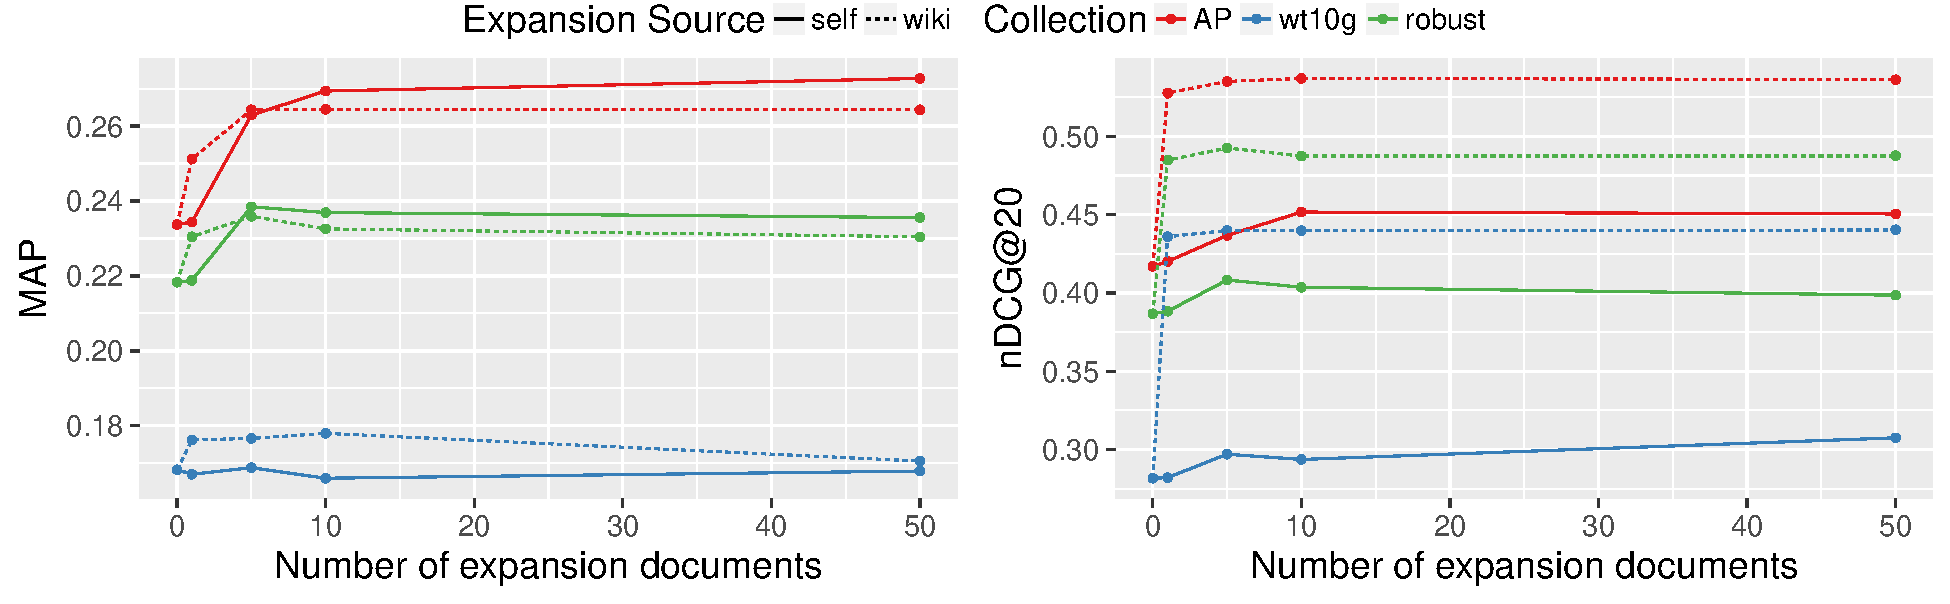
\includegraphics[width=\linewidth]{figures/expansion-sweep.pdf}
\caption{Sweeps over values of $n$, the number of expansion documents.}
\label{figure.n-sweeps}
\end{figure*}

\begin{table}
\begin{tabular}{|c|c|c|l|l|} \hline
{\bf Corpus} & {\bf \bigcell{l}{Exp. \\ Source}} & {\bf Run} & {\bf MAP} & {\bf nDCG@20} \\ \hline\hline
\rule{0pt}{2.5ex} \multirow{8}{*}{AP} & \cellcolor{gray!50} & \cellcolor{gray!50}{\it QL} & \cellcolor{gray!50}0.2337 & \cellcolor{gray!50}0.4170 \\ \cline{3-5}
\rule{0pt}{2.5ex} & \cellcolor{gray!50} \multirow{-2}{*}{\it Baseline} & \cellcolor{gray!50}{\it RM3} & \cellcolor{gray!50}0.3310$^\uparrow$ & \cellcolor{gray!50}0.4855$^\uparrow$ \\ \cline{2-5}
\rule{0pt}{2.5ex} & \multirow{2}{*}{\it Self} & {\it QL} & 0.2694$^\uparrow$ & 0.4519$^\uparrow$ \\ \cline{3-5}
\rule{0pt}{2.5ex} & & {\it RM3} & 0.3295$^{\uparrow *}$ & \textbf{0.4876}$^{\uparrow *}$ \\ \cline{2-5}
\rule{0pt}{2.5ex} & \multirow{2}{*}{\it Wiki} & {\it QL} & 0.2644$^\uparrow$ & 0.4582$^\uparrow$ \\ \cline{3-5}
\rule{0pt}{2.5ex} & & {\it  RM3} & 0.3334$^{\uparrow *}$ & 0.4811$^{\uparrow *}$ \\ \cline{2-5}
\rule{0pt}{2.5ex} & \multirow{2}{*}{\it Double} & {\it QL} & 0.2774$^{\uparrow SW}$ & 0.4734$^{\uparrow SW}$ \\ \cline{3-5}
\rule{0pt}{2.5ex} & & {\it RM3} & \textbf{0.3342}$^{\uparrow\Uparrow *S}$ & 0.4789$^\uparrow$ \\ \hline\hline
\rule{0pt}{2.5ex} \multirow{8}{*}{Robust} & \cellcolor{gray!50} & \cellcolor{gray!50}{\it QL} & \cellcolor{gray!50}0.2183 & \cellcolor{gray!50}0.3867 \\ \cline{3-5}
\rule{0pt}{2.5ex} & \cellcolor{gray!50} \multirow{-2}{*}{\it Baseline} & \cellcolor{gray!50}{\it RM3} & \cellcolor{gray!50}0.2639$^\uparrow$ & \cellcolor{gray!50}0.3908 \\ \cline{2-5}
\rule{0pt}{2.5ex} & \multirow{2}{*}{\it Self} & {\it QL} & 0.2369$^\uparrow$ & 0.4036$^\uparrow$ \\ \cline{3-5}
\rule{0pt}{2.5ex} & & {\it RM3} & 0.2591$^{\uparrow\Downarrow *}$ & 0.3894$^{*}$ \\ \cline{2-5}
\rule{0pt}{2.5ex} & \multirow{2}{*}{\it Wiki} & {\it QL} & 0.2326$^\uparrow$ & 0.4040$^\uparrow$ \\ \cline{3-5}
\rule{0pt}{2.5ex} & & {\it RM3} & \textbf{0.2674}$^{\uparrow *}$ & 0.4201$^{\uparrow\Uparrow *}$ \\ \cline{2-5}
\rule{0pt}{2.5ex} & \multirow{2}{*}{\it Double} & {\it QL} & 0.2417$^{\uparrow W}$ & 0.4156$^{\uparrow\Uparrow SW}$ \\ \cline{3-5}
\rule{0pt}{2.5ex} & & {\it RM3} & 0.2672$^{\uparrow *S}$ & \textbf{0.4205}$^{\uparrow\Uparrow S}$ \\ \hline\hline
\rule{0pt}{2.5ex} \multirow{8}{*}{wt10g} & \cellcolor{gray!50} & \cellcolor{gray!50}{\it QL} & \cellcolor{gray!50}0.1683 & \cellcolor{gray!50}0.2816 \\ \cline{3-5}
\rule{0pt}{2.5ex} & \cellcolor{gray!50} \multirow{-2}{*}{\it Baseline} & \cellcolor{gray!50}{\it RM3} & \cellcolor{gray!50}0.1651 & \cellcolor{gray!50}0.2834 \\ \cline{2-5}
\rule{0pt}{2.5ex} & \multirow{2}{*}{\it Self} & {\it QL} & 0.1660 & 0.2936 \\ \cline{3-5}
\rule{0pt}{2.5ex} & & {\it RM3} & 0.1694$^\Uparrow$ & 0.2758$^\Downarrow$ \\ \cline{2-5}
\rule{0pt}{2.5ex} & \multirow{2}{*}{\it Wiki} & {\it QL} & 0.1780$^\uparrow$ & 0.3029$^\uparrow$ \\ \cline{3-5}
\rule{0pt}{2.5ex} & & {\it RM3} & \textbf{0.2089}$^{\uparrow\Uparrow *}$ & \textbf{0.3085}$^{\uparrow\Uparrow}$ \\ \cline{2-5}
\rule{0pt}{2.5ex} & \multirow{2}{*}{\it Double} & {\it QL} & 0.1759$^{S}$ & 0.3148$^{\uparrow\Uparrow SW}$ \\ \cline{3-5}
\rule{0pt}{2.5ex} & & {\it RM3} & 0.2061$^{\uparrow\Uparrow *S}$ & 0.3082$^{\uparrow\Uparrow S}$ \\ \hline
\end{tabular}
\caption{Performance of runs using various expansion sources with (\textit{RM3}) and without (\textit{QL}) query expansion. Statistical significance at $p \leq 0.05$ is marked with a variety of symbols: $\uparrow$ indicates improvement over the baseline QL run; $\Uparrow$ and $\Downarrow$ indicate improvement and decline respectively with respect to the baseline RM3 run; $^{*}$ indicates improvement over the QL run with the same expansion source; $^{S}$ and $^{W}$ indicate improvement over the \textit{self} and \textit{wiki} sources, respectively, of the same run type. Bolded runs are the highest raw score for an evaluation metric in a given collection.}
\label{table.performance}
\end{table}

Retrieval performance of each run is shown in Table \ref{table.performance}. We measure performance with mean average precision (MAP) and normalized discounted cumulative gain at 20 (nDCG@20). Each metric is optimized with 10-fold cross-validation.

The results confirm that document expansion provides benefit over a baseline query likelihood run---no run performs significantly worse than the baseline, and most runs improve over the baseline QL run. % Note that baselines correspond to $\sum_{j=1}^n \lambda_{{\mathcal{E}_D}_j} = 0.0$. 

Performance of RM3 runs is more surprising with improvement over the baseline RM3 occurring more rarely compared to improvement over the baseline QL. The data suggest that RM3 runs may be more effective in more heterogeneous collections: there are three RM3 improvements in robust and six in wt10g, compared to only one in AP. This makes intuitive sense since a homogeneous collection would be expected to receive less benefit from query expansion. We can also see that an RM3 run typically improves over its QL counterpart, demonstrating that relevance modeling continues to operate effectively with the introduction of document expansion.

In general, \textit{wiki} runs perform similarly to \textit{double} runs. However, the strong performance of \textit{double} runs is visible when query expansion is ignored: five out of six \textit{double} QL runs show statistically significant improvement over \textit{wiki} QL runs. In one case (wt10g measuring nDCG@20) the \textit{double} QL run even outperforms the \textit{wiki} RM3 run with statistical significance.

\subsection{Sensitivity to \boldmath$n$}\label{section.n-sensitivity}

Figure \ref{figure.n-sweeps} shows sweeps over several values of $n$, the number of expansion documents, for each target collection using our established cross-validation procedure with identical folds. The sensitivity to $n$ is not pronounced at $n \geq 5$, and what little variation exists is not consistent across collections. We therefore choose the value of 10 as an apparently safe value; this is a convenient result since it allows for more efficient document expansion.

\section{Conclusions}\label{section.conclusions}

The results indicate that our approach for document expansion work well in general and especially in concert with traditional relevance modeling techniques. We find that we can improve on traditional document expansion by incorporating external collections into the expansion process. In the future, we plan to investigate in detail the relationship between homogeneity of documents and the performance of our model.

\section{Acknowledgments}\label{section.acknowledgments}
This work was supported in part by the US National Science Foundation under Grant No. [blind]. Any opinions, findings, conclusions, or recommendations expressed are those of the authors and do not necessarily reflect the views of the National Science Foundation.


\bibliographystyle{abbrv}
\bibliography{library}  

\end{document}
